\documentclass[tikz,border=6pt]{standalone}
\usepackage{tikz}
\usetikzlibrary{arrows.meta,positioning}
\begin{document}
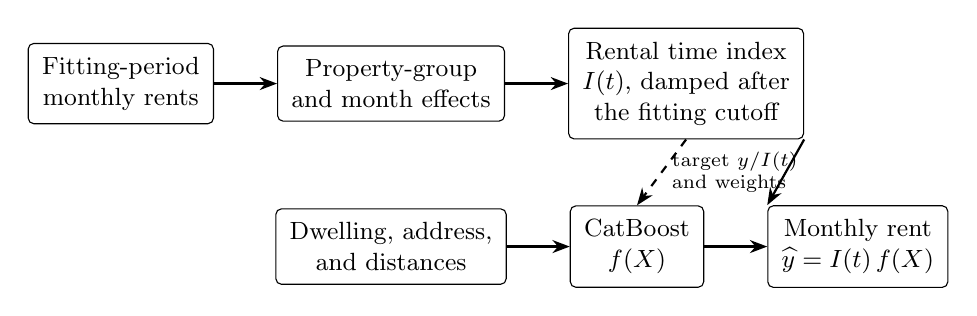
\begin{tikzpicture}[
  font=\small,
  box/.style={draw, rounded corners=2pt, align=center, inner sep=5pt},
  arr/.style={-{Stealth[length=2.2mm]}, thick},
  dasharr/.style={arr, dashed}
]
\node[box] (rent) {Fitting-period\\monthly rents};
\node[box, right=8mm of rent] (fe) {Property-group\\and month effects};
\node[box, right=8mm of fe] (idx) {Rental time index\\$I(t)$, damped after\\the fitting cutoff};
\node[box, below=11mm of fe] (x) {Dwelling, address,\\and distances};
\node[box, right=8mm of x] (tree) {CatBoost\\$f(X)$};
\node[box, right=8mm of tree] (y) {Monthly rent\\$\widehat y=I(t)\,f(X)$};
\draw[arr] (rent) -- (fe);
\draw[arr] (fe) -- (idx);
\draw[arr] (x) -- (tree);
\draw[arr] (tree) -- (y);
\draw[dasharr] (idx.south) -- node[right, font=\scriptsize, align=left] {target $y/I(t)$\\and weights} (tree.north);
\draw[arr] (idx.south east) -- (y.north west);
\end{tikzpicture}
\end{document}
